\documentclass[UTF8]{ctexart}

\usepackage{ctex}
\usepackage{times}
\usepackage{geometry}
\usepackage{subcaption}
\usepackage{textcomp}
\usepackage{tocbibind}
\usepackage{fancyhdr}
\usepackage{color}
\usepackage{graphicx}
\usepackage{titling}
\usepackage{hyperref}
\usepackage{fourier}
\usepackage{tabularx}
\usepackage{amssymb}
\usepackage{chemformula}
\usepackage{appendix}
\usepackage{multirow}
\usepackage{graphicx}
\usepackage{makecell}
\usepackage{adjustbox}
\usepackage{listings}
\usepackage{xcolor}
\usepackage{ulem}
\usepackage{enumitem}
\usetikzlibrary{arrows,positioning,shapes,patterns,calc}
\usepackage{booktabs}
\usepackage{float}
\usepackage{tikz}
\usepackage{tikz-timing}
\usepackage{algorithm}
\usepackage{algpseudocode}

% =====================================================================================
% Paper Define
% =====================================================================================

\hypersetup{
    colorlinks,
    linktoc=all,
    citecolor=black,
    filecolor=black,
    linkcolor=black,
    urlcolor=cyan
}

\geometry{a4paper,left=2cm,right=2cm,top=3cm,bottom=3cm}

\CJKfamily{\fangsong}

% 行内高亮
\lstdefinestyle{inlinecode}{
    basicstyle=\ttfamily\small,
    backgroundcolor=\colorbox{gray!10},
    breaklines=true,
    frame=none
}

\newcommand{\code}[1]{\colorbox{gray!10}{\lstinline[style=inlinecode]|#1|}}

% 行间高亮
\lstdefinestyle{codeblock}{
    basicstyle=\ttfamily\small,
    backgroundcolor=\color{gray!10},
    frame=single,
    frameround=tttt,
    framerule=0.5pt,
    rulecolor=\color{gray!50},
    breaklines=true,
    breakatwhitespace=false,
    numbers=left,
    numberstyle=\tiny\color{gray},
    stepnumber=1,
    numbersep=8pt,
    showspaces=false,
    showstringspaces=false,
    showtabs=false,
    tabsize=4,
    xleftmargin=15pt,
    xrightmargin=5pt,
    aboveskip=10pt,
    belowskip=10pt
}

\lstset{style=codeblock}

% 定义命令：双下划线 或者 波浪线
% \newcommand{\integrated}[1]{\uuline{#1}} % 双下划线
\newcommand{\integrated}[1]{\uwave{#1}} % 波浪线

\renewcommand{\algorithmicrequire}{\textbf{输入:}}
\renewcommand{\algorithmicensure}{\textbf{输出:}}

% =====================================================================================
% Header
% =====================================================================================

\pagestyle{fancy}
\fancyhead[L]{HTQ15-L DVP Protocol Specification}
\fancyhead[R]{Ver 1.1} % 版本号更新
\fancyfoot[C]{\thepage}

\begin{document}

% =====================================================================================
% Title
% =====================================================================================

\begin{center}
    \vspace*{1cm}
    {\Huge \textbf{HTQ15-L DVP传输协议规范}}
    \vspace{0.5cm}
    
    {\Large \textbf{HTQ15-L DVP Protocol Specification}}
    \vspace{2cm}
    
    \begin{tabular}{rl}
        \textbf{适用平台：} & Rockchip RK3588 / HTQ15-L \\
        \textbf{接口类型：} & 8-bit Parallel DVP (External Sync) \\
        \textbf{版本：} & v1.1 \\
        \textbf{日期：} & 2026-01-19 \\
    \end{tabular}
\end{center}

\vspace{2cm}

\newpage

% =====================================================================================
% Section 1: 概述
% =====================================================================================

\section{概述 (Overview)}

本协议旨在解决红外机芯在单通道 8-bit DVP 总线上同时传输 \textbf{8-bit YUV 图像数据} 与 \textbf{16-bit Raw 原始数据} 的需求。

鉴于 RK3588 VICAP 控制器及 FPGA 逻辑对“行长度固定 (Row Invariant)”的要求，本协议规定物理层传输带宽统一锁定为 \code{1280 Bytes/Line}。

\subsection{物理层参数}
\begin{itemize}
    \item \textbf{Pixel Clock (PCLK)}: Max 150MHz (RK3588 Limit).
    \item \textbf{Bus Width}: 8-bit.
    \item \textbf{Sync Mode}: External Sync (HREF/VSYNC/PCLK).
    \item \textbf{Physical Resolution}: $1280 \times H_{total}$ (高度取决于具体模式).
\end{itemize}

\newpage

% =====================================================================================
% Section 2: 协议模式
% =====================================================================================

\section{传输模式定义}

\subsection{模式 A: YUV422 (NV16) + Raw16 (推荐)}

此模式下，图像数据采用 \textbf{NV16 (Semi-Planar YUV422)} 格式。相比于 UYVY，NV16 将 Y 分量与 UV 分量分离存储，利于后续图像处理算法（如 ISP）直接读取。

由于物理行宽固定为 1280 Bytes，而逻辑行宽仅为 640 Bytes (8-bit)，因此在传输 Y 平面和 UV 平面时，采用\textbf{“双行合并”}策略。

\subsubsection{数据排布}

\begin{itemize}
    \item \textbf{Part 1 (Y Plane)}: 640 $\times$ 512 (8-bit)。
        \begin{itemize}
            \item \textbf{物理映射}: 逻辑 Line $2n$ 与 Line $2n+1$ 拼接。
            \item \textbf{物理行数}: $512 / 2 = \mathbf{256}$ Lines。
        \end{itemize}
    \item \textbf{Part 2 (UV Plane)}: 640 $\times$ 512 (8-bit Interleaved)。
        \begin{itemize}
            \item \textbf{物理映射}: 逻辑 Line $2n$ 与 Line $2n+1$ 拼接。
            \item \textbf{物理行数}: $512 / 2 = \mathbf{256}$ Lines。
        \end{itemize}
    \item \textbf{Part 3 (Raw Data)}: 640 $\times$ 512 Raw16。
        \begin{itemize}
            \item \textbf{物理映射}: 每个像素 2 Bytes，直接填满 1280 Bytes。
            \item \textbf{物理行数}: $\mathbf{512}$ Lines。
        \end{itemize}
    \item \textbf{Total Frame}: 物理分辨率 \textbf{1280 $\times$ 1024} ($256+256+512$)。
\end{itemize}

\begin{figure}[H]
    \centering
    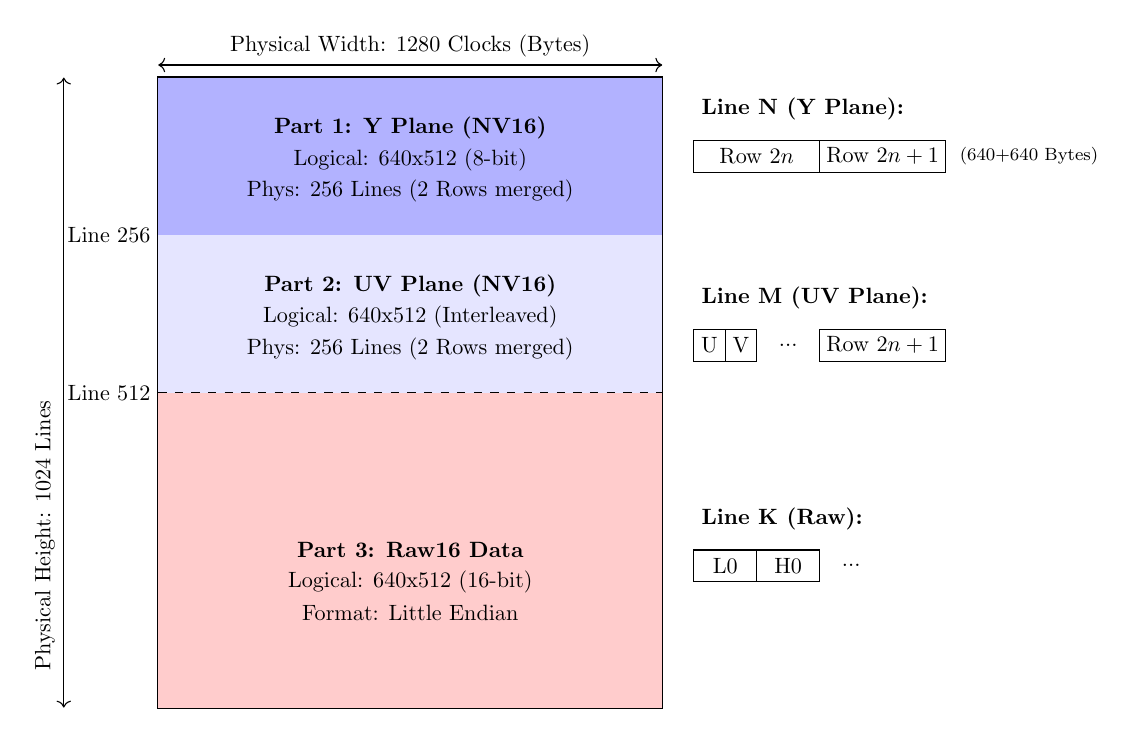
\begin{tikzpicture}[scale=0.8, every node/.style={transform shape}]
        % Draw Frame Box
        \draw[thick] (0,0) rectangle (8, 10);
        
        % Dimensions
        \draw[<->] (0, 10.2) -- (8, 10.2) node[midway, above] {Physical Width: 1280 Clocks (Bytes)};
        % yshift 保持，防止重叠
        \draw[<->] (-1.5, 0) -- (-1.5, 10) node[midway, left, rotate=90, yshift=0.3cm] {Physical Height: 1024 Lines};
        
        % --- Part 1: Y Plane ---
        \fill[blue!30] (0, 7.5) rectangle (8, 10);
        \node at (4, 9.2) {\textbf{Part 1: Y Plane (NV16)}};
        \node at (4, 8.7) {Logical: 640x512 (8-bit)};
        \node at (4, 8.2) {Phys: 256 Lines (2 Rows merged)};
        \draw[dashed] (0, 7.5) -- (8, 7.5);
        \node[anchor=east] at (0, 7.5) {Line 256};
        
        % --- Part 2: UV Plane ---
        \fill[blue!10] (0, 5) rectangle (8, 7.5);
        \node at (4, 6.7) {\textbf{Part 2: UV Plane (NV16)}};
        \node at (4, 6.2) {Logical: 640x512 (Interleaved)};
        \node at (4, 5.7) {Phys: 256 Lines (2 Rows merged)};
        \draw[dashed] (0, 5) -- (8, 5);
        \node[anchor=east] at (0, 5) {Line 512};
        
        % --- Part 3: Raw16 ---
        \fill[red!20] (0, 0) rectangle (8, 5);
        \node at (4, 2.5) {\textbf{Part 3: Raw16 Data}};
        \node at (4, 2) {Logical: 640x512 (16-bit)};
        \node at (4, 1.5) {Format: Little Endian};
        
        % --- Byte Stream Detail (Right Side) ---
        
        % Y Plane Detail
        \node[anchor=west] at (8.5, 9.5) {\textbf{Line N (Y Plane):}};
        \draw (8.5, 9) rectangle (10.5, 8.5); \node at (9.5, 8.75) {Row $2n$};
        \draw (10.5, 9) rectangle (12.5, 8.5); \node at (11.5, 8.75) {Row $2n+1$};
        \node[anchor=west] at (12.6, 8.75) {\footnotesize (640+640 Bytes)};

        % UV Plane Detail
        \node[anchor=west] at (8.5, 6.5) {\textbf{Line M (UV Plane):}};
        \draw (8.5, 6) rectangle (9.0, 5.5); \node at (8.75, 5.75) {U};
        \draw (9.0, 6) rectangle (9.5, 5.5); \node at (9.25, 5.75) {V};
        \node at (10, 5.75) {...};
        \draw (10.5, 6) rectangle (12.5, 5.5); \node at (11.5, 5.75) {Row $2n+1$};
        
        % Raw Detail
        \node[anchor=west] at (8.5, 3) {\textbf{Line K (Raw):}};
        \draw (8.5, 2.5) rectangle (9.5, 2); \node at (9, 2.25) {L0};
        \draw (9.5, 2.5) rectangle (10.5, 2); \node at (10, 2.25) {H0};
        \node at (11, 2.25) {...};
    \end{tikzpicture}
    \caption{Mode A: NV16 + Raw16 内存映射示意图}
\end{figure}

\subsection{模式 B: YUV420 (NV12) + Raw16 (低带宽)}

此模式用于降低带宽占用。利用 NV12 格式 Y 分量与 UV 分量分离的特性，将两行逻辑数据合并为一行物理数据传输。

\subsubsection{数据排布}

\begin{itemize}
    \item \textbf{Part 1 (Y Plane)}: 640 $\times$ 512 (8-bit)。每行 640 Bytes。
        \begin{itemize}
            \item \textbf{物理映射}: 将逻辑上的 Line $2n$ 和 Line $2n+1$ 拼接，组成一个 1280 Bytes 的物理行。
            \item \textbf{物理行数}: $512 / 2 = 256$ Lines。
        \end{itemize}
    \item \textbf{Part 2 (UV Plane)}: 640 $\times$ 256 (Interleaved)。每行 640 Bytes。
        \begin{itemize}
            \item \textbf{物理映射}: 同样两行拼一行。
            \item \textbf{物理行数}: $256 / 2 = 128$ Lines。
        \end{itemize}
    \item \textbf{Part 3 (Raw)}: 640 $\times$ 512 Raw16。
        \begin{itemize}
            \item \textbf{物理行数}: 512 Lines。
        \end{itemize}
    \item \textbf{Total Frame}: 物理分辨率 \textbf{1280 $\times$ 896} ($256+128+512$)。
\end{itemize}

\newpage

% =====================================================================================
% Section 3: 关键时序规范
% =====================================================================================

\section{关键时序规范 (Timing Specification)}

针对 RK3588 的 DVP 控制器特性，必须严格遵守以下时序约束，否则可能导致帧同步失败或错位。

\subsection{VSYNC 与 HSYNC 相位关系}

\textbf{禁止} VSYNC 与 HSYNC 的上升沿同时跳变。建议 VSYNC 提前 HSYNC 至少 4 个 PCLK 周期有效。

\begin{figure}[H]
    \centering
    \begin{tikztimingtable}[
        timing/slope=0.1,
        x=0.4cm, % 设置 X 轴单位长度
        y=0.8cm, % 设置 Y 轴单位长度
    ]
    PCLK   & 20{C} \\
    VSYNC  & 2L 14H 4L \\
    HSYNC  & 4L 10H 6L \\
    DATA   & 4U 10D{Valid Data} 6U \\
    \extracode
    \begin{pgfonlayer}{background}
        \vertlines[help lines]{2,4,14}
    \end{pgfonlayer}
    \end{tikztimingtable}
    \caption{DVP 帧开始 (Frame Start) 时序图}
\end{figure}

\subsection{时序参数表}

\begin{table}[H]
\centering
\begin{tabular}{@{}lccc@{}}
\toprule
\textbf{Parameter} & \textbf{Symbol} & \textbf{Value (Clocks)} & \textbf{Note} \\ \midrule
Horizontal Active & $H_{act}$ & 1280 & Fixed \\
Horizontal Blanking & $H_{blk}$ & $\ge 48$ & Min requirement \\
Vertical Active & $V_{act}$ & 1024 (Mode A) / 896 (Mode B) & \\
Vertical Front Porch & $V_{fp}$ & $\ge 2$ Lines & \\
Vertical Back Porch & $V_{bp}$ & $\ge 2$ Lines & \\ \bottomrule
\end{tabular}
\caption{时序参数约束}
\end{table}

\newpage

% =====================================================================================
% Section 4: 软件解析伪代码
% =====================================================================================

\section{接收端解析逻辑}

RK3588 接收到的将是一个宽为 1280 的大图，应用层需通过指针偏移还原数据。

\begin{algorithm}[H]
    \caption{Mode A (NV16) 数据解析逻辑}
    \begin{algorithmic}[1]
        \Require 缓冲区指针 $Buffer$, 图像宽度 $W=640$, 图像高度 $H=512$
        \Ensure 指向 Y、UV、Raw 数据的指针
        
        \State \textbf{常量定义:}
        \State \quad $W_{phys} \gets 1280$ \Comment{物理行宽 (Bytes)}
        \State \quad $H_{y\_phys} \gets 256$ \Comment{Y平面物理高度 (512/2)}
        \State \quad $H_{uv\_phys} \gets 256$ \Comment{UV平面物理高度 (512/2)}
        
        \Statex
        \State \textbf{步骤 1: 定位 Y Plane (NV16)}
        \State $Ptr_{Y} \gets Buffer$
        \State \Comment{注意：逻辑行 $2n$ 在物理行前半段，逻辑行 $2n+1$ 在后半段}
        
        \Statex
        \State \textbf{步骤 2: 定位 UV Plane (NV16)}
        \State $Offset_{uv} \gets W_{phys} \times H_{y\_phys}$
        \State $Ptr_{UV} \gets Buffer + Offset_{uv}$
        
        \Statex
        \State \textbf{步骤 3: 定位 Raw16 数据}
        \State $Offset_{raw} \gets Offset_{uv} + (W_{phys} \times H_{uv\_phys})$
        \State $Ptr_{Raw} \gets Buffer + Offset_{raw}$
        
        \Statex
        \Function{GetRawPixel}{$x, y$}
            \State $Index \gets y \times 640 + x$
            \State \Return $Ptr_{Raw}[Index]$
        \EndFunction
    \end{algorithmic}
\end{algorithm}

\end{document}